\begin{atiTask}[
  title = Verifikation des Greenschen Satzes
]
Berechnen Sie das Integral
\[
\oint_C \left(xy\D x+ x^2\D y\right),
\]
wobei der Integrationsweg $C$ aus den Seiten des Quadrates mit den Eckpunkten $A(0,0)$, $B(1,0)$, $C(1,1)$ und $D(0,1)$ besteht und entgegen dem Uhrzeigersinn durchlaufen wird. Verwandeln Sie dann das Kurvenintegral in ein Doppelintegral und verifizieren Sie den Greenschen Satz.

\end{atiTask}
\begin{atiSolution}
	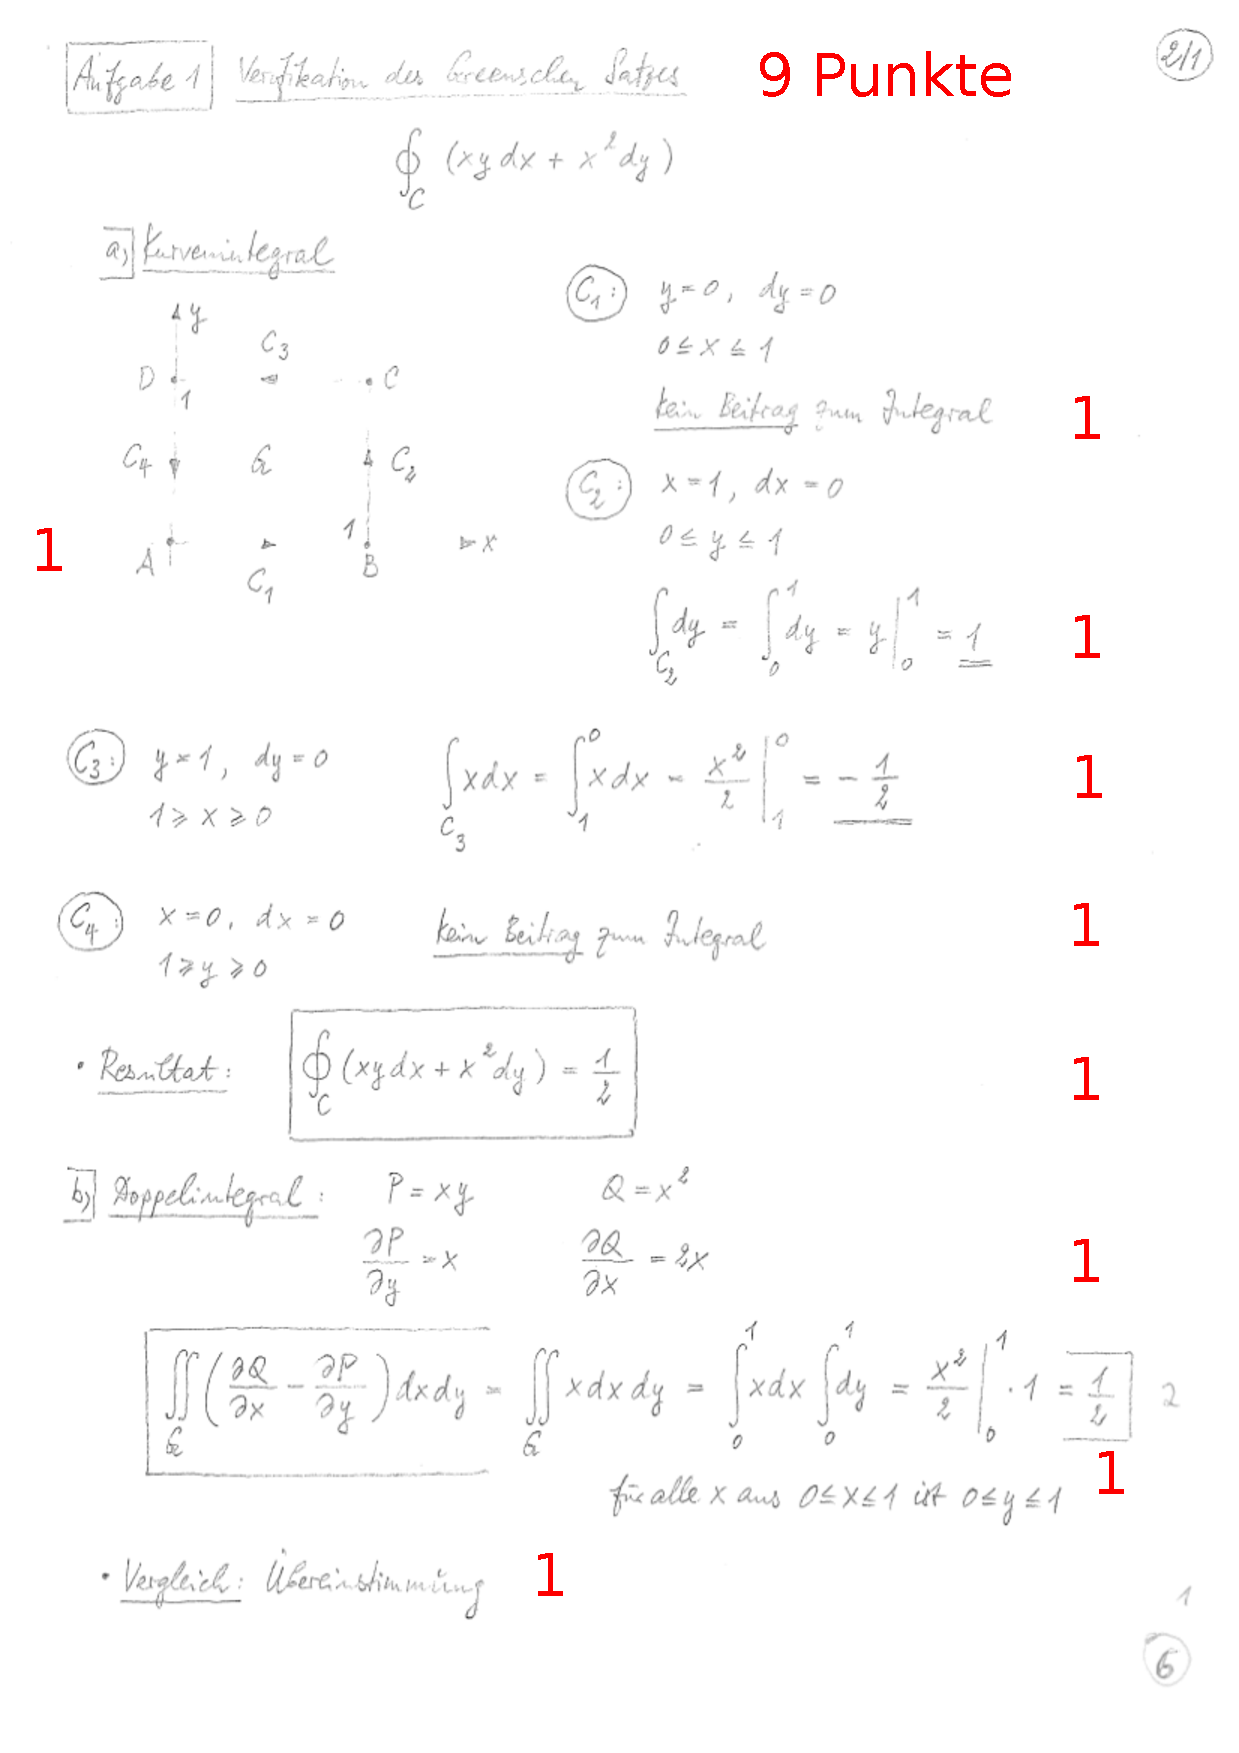
\includepdf{solution-green2D_i.pdf}}
\end{atiSolution}